\documentclass{scrartcl}
% \usepackage{hyperref}
% \usepackage{tikz}
\usepackage{amsmath}
\usepackage{amsthm}
\usepackage{pifont}
\usepackage{mathrsfs}
\usepackage{amssymb}
\usepackage{xcolor}
\usepackage{colortbl}
\usepackage{tikz-cd}
\usepackage{caption}
\usepackage{newunicodechar}


\usepackage[utf8]{inputenc}
\usepackage{ucs}
% \DeclareUnicodeCharacter{03A3}{\ensuremath{\Sigma}}



\usetikzlibrary{positioning,shapes.geometric,fit,arrows.meta}


\captionsetup{justification=centering}



\usepackage{booktabs}

\usepackage{hyperref}
% \usepackage{tikz}
\usepackage{amsmath}
\usepackage{amsthm}
\usepackage{pifont}
\usepackage{mathrsfs}
\usepackage{amssymb}
\usepackage{xcolor}
\usepackage{colortbl}
\usepackage{tikz-cd}
\usepackage{caption}
\usepackage{newunicodechar}


\usepackage[utf8]{inputenc}
\usepackage{ucs}
% \DeclareUnicodeCharacter{03A3}{\ensuremath{\Sigma}}



\usetikzlibrary{positioning,shapes.geometric,fit,arrows.meta}


\captionsetup{justification=centering}



\definecolor{darkgreen}{rgb}{0.0, 0.5, 0.0}

\newcommand{\tto}{\twoheadrightarrow}
\newcommand{\sse}{\subseteq}
\newcommand{\bset}{\mathbf{Set}}
\newcommand{\nat}{\mathbb{N}}

% Comments
\newcommand{\sacomment}[1]{\textcolor{green}{#1}}
\newcommand{\apcomment}[1]{\textcolor{blue}{#1}}
\newcommand{\greyout}[1]{\textcolor{gray}{#1}}
\newcommand{\err}[1]{\textcolor{red}{#1}}

% Theorem style
% \newtheorem{thm}{Theorem}
% \newtheorem{dfn}[thm]{Definition}
% \newtheorem{prop}[thm]{Proposition}
% \newtheorem{cor}[thm]{Corollary}
% % \newtheorem{lemma}[thm]{Lemma}
% % \newtheorem{rmk}[thm]{Remark}
% % \newtheorem{expl}[thm]{Example}
% \newtheorem{notn}[thm]{Notation}
% %\theoremstyle{nonumberplain}
% %\theoremsymbol{\Box}
% % \newtheorem{proof}{Proof}

\newcommand{\RP}{\mathrm{RP}}
\newcommand{\gRP}{\mathbf{RP}}
\newcommand{\RPm}{\mathrm{RP^{-}}}
\newcommand{\gRPm}{\mathbf{RP^{-}}}
\newcommand{\NF}{\mathrm{NF}}
\newcommand{\MF}{\mathrm{MF}}
\newcommand{\UN}{\mathrm{UN}}
\newcommand{\gUN}{\mathbf{UN}}
\newcommand{\UNto}{\mathrm{UN}^{\to}}
\newcommand{\gUNto}{\mathbf{UN}^{\to}}
\newcommand{\SN}{\mathrm{SN}}
\newcommand{\gSN}{\mathbf{SN}}
\newcommand{\decSN}{\mathrm{dec(SN)}}
\newcommand{\SM}{\mathrm{SM}}
\newcommand{\SMseq}{\mathrm{SMseq}}
\newcommand{\gSMseq}{\mathbf{SMseq}}
\newcommand{\gSM}{\mathbf{SM}}
\newcommand{\WN}{\mathrm{WN}}
\newcommand{\gWN}{\mathbf{WN}}
\newcommand{\SMandWN}{\mathrm{SM\land WN}}
\newcommand{\gSMandWN}{\mathbf{SM\land WN}}
\newcommand{\WM}{\mathrm{WM}}
\newcommand{\gWM}{\mathbf{WM}}
\newcommand{\WNFP}{\mathrm{WNFP}}
\newcommand{\NP}{\mathrm{NP}}
\newcommand{\gNP}{\mathbf{NP}}
\newcommand{\NPe}{\mathrm{NP_=}}
\newcommand{\gNPe}{\mathbf{NP_=}}
\newcommand{\WMFP}{\mathrm{WMFP}}
\newcommand{\MP}{\mathrm{MP}}
\newcommand{\gMP}{\mathbf{MP}}
\newcommand{\CR}{\mathrm{CR}}
\newcommand{\CRs}{\mathrm{CR^{\le 1}}}
\newcommand{\gCRs}{\mathbf{CR^{\le 1}}}
\newcommand{\gCR}{\mathbf{CR}}
\newcommand{\WCR}{\mathrm{WCR}}
\newcommand{\gWCR}{\mathbf{WCR}}
\newcommand{\Inc}{\mathrm{Inc}}
\newcommand{\gInc}{\mathbf{Inc}}
% \newcommand{\BP}{\mathrm{BP}}
\newcommand{\gBP}{\mathbf{BP}}
\newcommand{\FB}{\mathrm{FB}}
\newcommand{\CP}{\mathrm{CP}}
\newcommand{\gCP}{\mathbf{CP}}



\newcommand{\from}{\leftarrow}



\newcommand{\red}[1]{\textcolor{red}{#1}}
\newcommand{\blue}[1]{\textcolor{blue}{#1}}

% Reduction relation macros
\newcommand{\rstep}{\mathbin{\longrightarrow_R}}
\newcommand{\mstep}{\mathbin{\longrightarrow_R^*}}
\newcommand{\estep}{\mathbin{\longrightarrow_R^=}}
\newcommand{\rrstep}{\mathbin{\longrightarrow_R^r}}
\newcommand{\brstep}{\mathbin{\longleftarrow_R^r}}
\newcommand{\bstep}{\mathbin{\longleftarrow_R}}
\newcommand{\bmstep}{\mathbin{\longleftarrow_R^*}}

% Unicode characters

\newunicodechar{∀}{\ensuremath{\forall}}
\newunicodechar{→}{\ensuremath{\rightarrow}}
\newunicodechar{ℕ}{\ensuremath{\mathbb{N}}}
\newunicodechar{↔}{\ensuremath{\leftrightarrow}}
\newunicodechar{⊆}{\ensuremath{\sse}}
\newunicodechar{∧}{\ensuremath{\land}}
\newunicodechar{₌}{\ensuremath{_=}}
\newunicodechar{𝓟}{\ensuremath{\mathcal{P}}}
\newunicodechar{∈}{\ensuremath{\in}}
\newunicodechar{φ}{\ensuremath{\phi}}
\newunicodechar{Σ}{\ensuremath{\Sigma}}
\newunicodechar{₁}{\ensuremath{{}_1}}


% Misc Macros
\newcommand{\terese}{[TeReSe]}
% \newcommand{\ul}[1]{\underline{#1}}
\newcommand{\ule}[1]{\underline{#1:}}
% \newcommand{\setof}[1]{\{#1\}}
\newcommand{\setof}[1]{\left\{#1\right\}}


\newcommand{\tclos}[1]{{#1}^{\scriptscriptstyle{+}}}


% Taken from well founded section

\newcommand{\isWFacc}{\mathtt{isWFacc}}
\newcommand{\isWFseq}{\mathtt{isWFseq}}
\newcommand{\isWFmin}{\mathtt{isWFmin}}
\newcommand{\isWFaccm}{\mathtt{isWFacc-}}
\newcommand{\isWFseqm}{\mathtt{isWFseq-}}
\newcommand{\isWFminm}{\mathtt{isWFmin-}}

\newcommand{\isMinDec}{\mathtt{isMinDec}}


\title{Summer 2024 Report}
\author{Sam Arkle}
\date{\today}


\usepackage{pifont}% http://ctan.org/pkg/pifont
\newcommand{\cmark}{\quad\ding{51}}%
\newcommand{\xmark}{\quad\ding{55}}%

\newcommand{\thra}{\twoheadrightarrow}
\newcommand{\thla}{\twoheadleftarrow}
\newcommand{\thlra}{{\thla\!\!\thra}}

\newcommand{\down}[1]{{#1}{\downarrow}}
\begin{document}
\renewcommand{\arraystretch}{1.3}

\maketitle

\tableofcontents

\section{Introduction}
This is a report on the progress I have made during the summer of 2024 working with Dr. Polonsky \footnote{Assisstant Professor, Department of Computer Science, Appalachian State University.}. I have been writing on the topic of relations, working primarily from Term Rewriting Systems (TeReSe) \footnote{(Term Rewriting Systems. (2003). United Kingdom: Cambridge University Press.)}.
The objective of this work has been to both develop a formal understanding of relations and to build a library in Agda \footnote{\href{https://github.com/DrPolonsky/LAM/tree/main/Relations}{Github repository for this project's code}} that will be used as a foundation to further work in theoretical computer science.
\\
I have been focussed on Chapter 1 of TeReSe which covers abstract reduction systems (ARS) as well as the appendix (sections 1-3) which provides the necessary mathematical background for the rest of the book (e.g. relations, ordinals, inductive definitions and the Knaster-Tarski lemma). Where the book has made use of classical logic I have investigated the possibility of using constructive alternatives.

\section{Definitions} \label{section:Definitions}
The most interesting work we have carried out in investigating Chapter 1 of TeReSe has resulted from trying to provide constructive proofs for Newman's lemma, the Knaster-Tarski lemma, theorem 1.2.2 and theorem 1.2.3. Before exploring those proofs the following definitions are essential.


The following definitions are taken from [TeReSe], Chapter 1,
with minimal adaptations for consistency.

\begin{dfn}
  An abstract reduction system (\emph{ARS}) is a structure $\mathcal{A} = (A, R_\alpha)$ where $A$ is a set and $R_\alpha$ is a set of binary relations.
\end{dfn}
A relation $R$ from the set $R_\alpha$ is refered to as a reduction (or rewrite) relation. For example, if we specify $R$ as the relation of being 'less than' ($<$) then $R\, 4\, 2$. \textcolor{red}{Right?}
\apcomment{Yes, but move this to a(n eventual) list of examples.}

We use $R$ or $\to$ for a single-step reduction and $R^*$ or $\tto$ for a multi-step reduction.

\sacomment{Should we be using $R^+$ rather than $R^*$?}

\apcomment{Thus, when $(a,b) \in \to_{(\alpha)}$, we say that there is a
\emph{$(\alpha-)$reduction} from $a$ to $b$.
When $(a,b) \in \tto_\alpha$, we say that there is a multi-step $\alpha$-reduction
from $a$ to $b$.}

\begin{dfn}
  An element $a \in A$ is \emph{R-weakly confluent} ($WCR_R$) if all single step reductions from $a$ can always converge
  via multi-step reductions to some common reduct.
  A relation $R$ is \emph{weakly confluent} (AKA weakly Church-Rosser (WCR)) if every $a \in A$ is R-weakly confluent.
\end{dfn}

\begin{dfn}
  An element $a \in A$ is \emph{R-confluent} ($CR_R$) if all multi-step reductions from $a$ can always converge
  via multi-step reductions to some common reduct.
  A relation $R$ is \emph{confluent} (AKA Church-Rosser (CR)) if every $a \in A$ is R-confluent.
\end{dfn}

\begin{figure}[h]
  \centering
\[  \begin{tikzpicture}[node distance=1.5cm, auto]
    % Nodes
    \node (top) {a};
    \node (left) [below left of=top] {b};
    \node (right) [below right of=top] {c};
    \node (bottom) [below right of=left] {d};

    % Arrows
    \draw[->] (top) -- (left);
    \draw[->] (top) -- (right);
    \draw[->>] (left) -- (bottom);
    \draw[->>] (right) -- (bottom);
\end{tikzpicture}
\hspace{3cm}
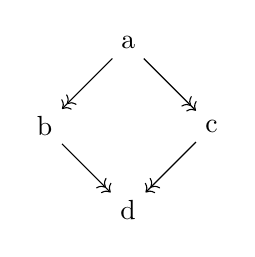
\begin{tikzpicture}[node distance=1.5cm, auto]
  % Nodes
  \node (top) {a};
  \node (left) [below left of=top] {b};
  \node (right) [below right of=top] {c};
  \node (bottom) [below right of=left] {d};

  % Arrows
  \draw[->>] (top) -- (left);
  \draw[->>] (top) -- (right);
  \draw[->>] (left) -- (bottom);
  \draw[->>] (right) -- (bottom);
\end{tikzpicture}
\]
\caption{On the left is an example of a weakly confluent relation. On the right is an example of a confluent relation.}
\end{figure}


\begin{dfn}
  \emph An element $a \in A$ is a {normal form} if there exists no reduction to any other element in $A$.
\end{dfn}

\begin{dfn}
  An element $a \in A$ is \emph{$R$-weakly normalizing} ($WN_{R}$)if $a \tto b$ for some normal form $b \in A$.

  A relation $R$ is weakly normalizing (WN) if every $a \in A$ is $R$- weakly normalizing.
\end{dfn}

\begin{dfn}
  An element $a \in A$ is \emph{$R$-strongly normalizing} ($SN_R$) if every reduction sequence starting from $a$ is finite.

  A relation $R$ is strongly normalizing (SN) if every
  $a \in A$ is $R$-strongly normalizing.
\end{dfn}

The above definition of SN is taken from [TeReSe]. When working in Agda, we make use of the alternative definition presented in [TeReSe] ($\leftarrow$ is accessibly well-founded).

\subsection{Closure operations on relations}

A relation $R$ has the following properties when the stated conditions are met:
\begin{dfn}
  \emph{reflexive} {- $\forall x \in A : x \to x $}
\end{dfn}
\begin{dfn}
  \emph{transitive} {- $\forall x, y, z \in A : ( x \to y \land y \to z ) \implies x \to z $}
\end{dfn}
\begin{dfn}
  \emph{symmetric} {- $\forall x, y \in A : x \to y \implies y \to x$}
\end{dfn}

\begin{dfn}
  The \emph{closure} of $R$ is the smallest relation that contains $\to$ and satisfies a given property.
\end{dfn}

\begin{dfn}
  The \emph{reflexive closure} of $R$ is the smallest relation $\to^r$ that contains $\to$ and is reflexive.
\end{dfn}
\begin{dfn}
  The \emph{symmetric closure} of $R$ is the smallest relation $R^s$ that contains $R$ and is symmetric.
\end{dfn}
\begin{dfn}
  The \emph{transitive closure} of $R$ is the smallest relation $R^+$ that contains $R$ and is transitive.
\end{dfn}
\begin{dfn}
  The \emph{reflexive transitive closure} of $R$ is the smallest relation $R^*$ that contains $R$ and is both reflexive and transitive.
\end{dfn}
\begin{dfn}
  The \emph{equivalence relation} of $R$ is the smallest relation $R^=$ that contains $R$ and is reflexive, transitive, and symmetric.
\end{dfn}

\begin{dfn}
  A relation $R$ has the \emph{weak normal form property} (WNFP) if
 $a \tto b$ and $a \tto c$  $\implies$
 $c \tto b$, for all $a,c \in A$ and all normal form $b \in A$.
\end{dfn}


\begin{dfn}
  A relation $R$ has the \emph{normal form property} (NFP) if
 $a \to^= b$  $\implies$
 $a \tto b$, for all $a \in A$ and any normal form $b \in A$.
\end{dfn}

Two elements $a, b \in A$ being equivalent is denoted $a \equiv b$.

\begin{dfn}
  A relation $R$ has the \emph{unique normal form property} (UN) if
  $a \to^= b$  $\implies$
  $a \equiv b$, for all $a \in A$ and any normal form $b \in A$.
\end{dfn}

\begin{dfn}
  A relation $R$ has the \emph{unique normal form property with respect to reduction} (UN$^ \to$) if
  $a \twoheadleftarrow  \cdot  \tto b$  $\implies$ $a \equiv b$, for all normal forms $a,b \in A$.
\end{dfn}

Let $A$ be a set.
\begin{dfn}
  A \emph{sequence (in $A$)} is a function from the natural numbers to $A$:
  \begin{align*}
    &s : \nat \to A \\
    &s = (s_0,s_1,s_2,\dots)
  \end{align*}
\end{dfn}

\begin{dfn}
  A sequence is \emph{$R$-increasing} if every term is $R$-related to its preceding term.
\end{dfn}

\begin{dfn}
  A sequence is \emph{bounded} if there exists an element $a$ to which all elements of the sequence reduce.
\end{dfn}

\begin{figure}[h]
  \centering
  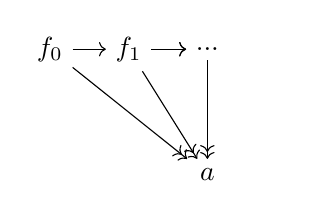
\begin{tikzpicture}
      % Define the nodes inside the region f
      \node (f0) at (0, 0) {$f_0$};
      \node (f1) at (1, 0) {$f_1$};
      \node (dots) at (2, 0) {$...$};

      % Draw the arrows between the nodes inside the region f
      \draw[->] (f0) -- (f1);
      \draw[->] (f1) -- (dots);
      \draw[->] (f1) -- (dots);


      % Define the nodes outside the region f
      \node (a) [below=of dots, yshift=-.25cm] {\parbox{2cm}{\centering $a$ }};

          % Draw the arrows between the nodes inside and outside the region f sds

          \draw[->>] (f0) -- (a);
          \draw[->>] (f1) -- (a);
          \draw[->>] (dots) -- (a);
      \end{tikzpicture}
      \caption{An example of a bounded sequence.}

    \end{figure}


\begin{dfn}
  An element $a \in A$ has the \emph{recurrence property} if $a \tto b \implies b \tto a$ for all $b \in A$.
\end{dfn}
\sacomment{I've been using $\tto$ as interchangable with $R *$ (as in the above definition).
Is that okay or am I going to have to clarify why they are interchangable (are they not interchangable?)?}
\apcomment{It's okay, but later we will need to make sure we are using them consistently.  Say that in Agda code, $\to$ is denoted by $R$.}

\begin{dfn}
  A relation $R$ has the \emph{recurrence property} (RP) if every
  bounded, increasing sequence has a recurrent element.
\end{dfn}

    \begin{figure}[h]
      \centering
      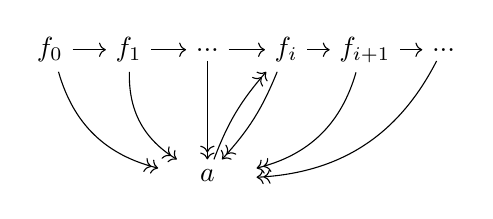
\begin{tikzpicture}
          % Define the nodes inside the region f
          \node (f0) at (0, 0) {$f_0$};
          \node (f1) at (1, 0) {$f_1$};
          \node (dots) at (2, 0) {$...$};
          \node (fi) at (3, 0) {$f_i$};
          \node (fi+1) at (4, 0) {$f_{i+1}$};
          \node (dots2) at (5,0) {$...$};

          % Draw the arrows between the nodes inside the region f
          \draw[->] (f0) -- (f1);
          \draw[->] (f1) -- (dots);
          \draw[->] (dots) -- (fi);
          \draw[->] (fi) -- (fi+1);
          \draw[->] (fi+1) -- (dots2);


          % Define the nodes outside the region f
          \node (a) [below=of dots, yshift=-.25cm] {\parbox{1cm}{\centering $a$ }};

              % Draw the arrows between the nodes inside and outside the region f sds

              \draw[->>] (f0) to [bend right] (a);
              \draw[->>] (f1) to [bend right] (a);
              \draw[->>] (dots) -- (a);
              \draw[->>] (fi) to [bend left=10] (a);
              \draw[->>] (fi+1) to [bend left] (a);
              \draw[->>] (dots2) to [bend left] (a);
              \draw[->>] (a) to [bend left=10] (fi);

          \end{tikzpicture}
          \caption{An example of a relation with the recurrence property.}

        \end{figure}
\begin{dfn}
  A relation $R$ has the \emph{weak recurrence property} (RP-) if
  for every increasing sequence with bound $a$,
  there is an element $i$ of the sequence such that $a \tto f (i)$.
\end{dfn}

\begin{dfn}
  A relation $R$ has the \emph{recurrence property} (RP) if
 $a \tto b$ and $a \tto c$  $\implies$
 $c \tto b$, for all $a,c \in A$ and all $b \in A$ with the recurrence property.
\end{dfn}
\sacomment{This mirrors our Weak normal form property but for recurrence. Which would be a suitable name?}

\begin{dfn}
  An element $a \in A$ is \emph{$R$-weakly recurrent} ($WR_{R}$)if $a \tto b$ for some recurrent element $b \in A$.

  A relation $R$ is weakly recurrent (WR) if every $a \in A$ is $R$- weakly recurrent.
\end{dfn}

\begin{dfn}
  An element $a \in A$ is \emph{$R$-strongly recurrent} ($SR_R$) if every reduction sequence starting from $a$ reaches a recurrent element in a finite number of reductions.

  A relation $R$ is strongly recurrent (SR) if every
  $a \in A$ is $R$-strongly recurrent.
\end{dfn}
\sacomment{Not sure on this defn. Is it right to state it requires a finite number of steps}







\begin{dfn}
  \emph{Cofinality property}
\end{dfn}
\sacomment{Still not sure on how to define cofinality.}

\begin{dfn}
  A relation $R$ is \emph{finitely branching} (FB) if, for all $a \in A$, the set of one step reducts of $a$ is finite.
\end{dfn}

\subsection{Recurrence property and increasing relations}

In [TeReSe], a relation $R \sse A \times A$ is called \emph{increasing} if there
exists a ``size function'' $|-| : A \to \nat$ satisfying, for all $x, y \in A$,
 \[ Rxy \to |x| < |y| \]

\begin{prop}
  If $R$ is increasing, then no infinite $R$-increasing sequence is bounded.
\end{prop}
\begin{proof}
  Let $(a_i) = a_0 \to a_1 \to a_2 \to \cdots$ be an $R$-increasing sequence
  and suppose that $(a_i)$ is bounded.  Let $b$ be the bound, so that $a_i \to b$ for all $i$.

  If $m = |b|$ then we have
  \[ 0 \le |a_0| < |a_1| < |a_2| < \cdots < |a_m| < |b| = m \]
  % \[ m > |a_m| > |a_{m-1}| > \cdots > |a_0| \ge 0 \]
  which is a contradiction, since there are only $m-1$ integers strictly less than $m$.
\end{proof}

It follows that every relation that is increasing in the sense of [TeReSe]
vacuously satisfies the RP condition.

\begin{cor}
  If $R$ is increasing, then $R$ has the recurrence property.
\end{cor}


\section{Classical Principles}
Principles we are considering
\begin{itemize}
  \item Decidability of equality on $A$
  \item Decidability of the relation $R$
  \item When relevant, decidability of the given precicate $P$
  \item Not-not-closure of being accessible
  \item Not-not-closure of $R$
  \item Not-not-closure of $P$
  \item Decidability of whether a given element is an $R$-normal form
  \item When relevant, local/element-wise versions of the above
  \item Markov's principle:
  \begin{itemize}
    \item In $wfMin_0 \to wfSeq$.

    Given a sequence $s : \nat \to A$, let $E(a) = \exists n \in \nat. s n \equiv a$.

    Need: $\forall a. \lnot\lnot E(a) \to E(a)$, i.e.,
    \[\lnot\lnot \big(\exists n \in \nat. s n \equiv a\big)
          \to \big(\exists n \in \nat. s n \equiv a\big)\]

  \end{itemize}
\end{itemize}

\section{Implications}
{\small
We now look into the interrelation of the various properties defined in Section~\ref{section:Definitions}. Our aim is to expand on the
connections made in Figure 1.8 of [TeReSe] (p.19).

The following are the implications we have proven in Agda, along with a reference to the name of the proof in Agda. Where appropriate we indicate
which classical assumptions were used as part of the proof.

\begin{itemize}
  \item SN and WCR $\implies$ CR

\texttt{NewmansLemma : $\mathnormal{\forall}$ \{R : $\mathbb{R}$ A\} $\to$ SN R $\to$ weakly-confluent R $\to$ confluent R}


We have also provided a proof elementwise making use of the classical principal
about the decidability of $R$ being minimal.


\texttt{SN$\land$UN$\to$CRelem :\newline $\forall$ (R : $\mathbb{R}$ A) $\to$ decMin (~R R) $\to$ $\forall$ x $\to$ is R -SN x $\to$ is R -UN x$\to$ is R -CR x}

\sacomment{How to one line this consistently and in a pretty way?}

\item{CP $\implies$ CR}

\texttt{iv : CP R $\to$ confluent R}

This is theorem 1-2-3 iv in [TeReSe]

\item{WN and UN $\implies$ CR}

\texttt{ii : WN R $\times$ UN R $\to$ confluent R}

This is theorem 1-2-2 ii in [TeReSe]

\item{WN and UN $\implies$ bounded}

\texttt{i : WN R $\to$ UN R $\to$ bounded R}

\sacomment{Going to have to find a way to neatly represent the implications}


\sacomment{note to self, tidy up below with references to agda code}

\item{WN and UN$\to$ $\implies$ bounded}

\texttt{i+ : WN R $\to$ UN$\to$ R $\to$ bounded R}

\item{WN and UN and RP $\implies$ wfSeq - ($\sim$ R)}

\texttt{ii3- :  WN R $\to$ UN R $\to$ RP R $\to$ isWFseq- ($\sim$R R)}

\item {CR $\implies$ WCR}

\texttt{CR$\to$WCR : CR R $\to$ WCR R }

\item {NF $implies$ UN}
\sacomment{Need to prove}

\item {SN and WCR $\implies$ UN and WN}
\sacomment{Need to proove}
\texttt{}

\item {Ind and Inc $\implies$ SN} \sacomment{I don't think we have
a proof of this, should we include it, include it with a note that we're taking [TeReSe]'s word on it?}


\item {WCR, WN, and, Inc $\implies$ SN}


\item {WCR, WN, and RP $\implies$ SN}


\item {CR $\implies$ NF $\implies$ UN}

\texttt{i-4 : confluent R $\to$ NFP R $\to$ UN R}

\item {CR $^{\leq1} \implies$ CR}

\texttt{iv : CP R $\to$ confluent R}

\end{itemize}
}

\subsection{Summary table}
BP = boundedness property

Table listing highest "confluence" property implied
by the conjunction of row and column.


\begin{tabular}{@{}l@{\quad}l@{\quad}l@{\quad}l@{\quad}l@{\quad}l@{}}
  \toprule
  & CP & CR & WCR & WNFP & WUN  \\
  \midrule
  SN  & ? & CR & CR & (Should be CR?)  & ?  \\
  WN  & ? & CR & (Not CR) & ? & ? \\
  WN* & ? & CR & ? & ? & ? \\
  BP $\land$ CP & ? & CR & ? & ? & ? \\
  BP  & ? & CR & ? & ? & ? \\
  CP  & ? & CR & ? & ? & ? \\
  \bottomrule
\end{tabular}


Table listing highest "normalization" property implied
by the conjunction of row and column.


\begin{tabular}{@{}l@{\quad}l@{\quad}l@{\quad}l@{\quad}l@{\quad}l@{}}
  \toprule
  & CP & CR & WCR & WNFP & WUN \\
  \midrule
  SN  &?& SN & SN & SN & SN \\
  WN  &?& (Not SN) & (Not SN) & ? & ? \\
  WN*  &?& ? & ? & ? & ? \\
  BP $\land$ CP   &?& ? & ? & ? & ? \\
  BP  &?& ? & ? & ? & ? \\
  CP  &?& (not CP or BP) & ? & ? & ? \\
  \bottomrule
\end{tabular}

\subsection{Double-check: What has been proven}
\begin{itemize}
  \item \sacomment{List all the constructive proofs we've put together!}
  \item SN implies bounded
  \item RP- implies RP
  \item The infinite haircomb refutes $WN \land RP \to \omega$-bounded.  But it is not WCR.
  \item We have formalized proposition 1.1.9, 1.1.10, 1.1.11 from [TeReSe].
  \item We have a proof for Theorem 1.2.1 (Newlman's Lemma) (though we have just one proof of multiple possible proofs).
  \item We have a proof for all parts of Theorem 1.2.2
  \item We have a proof for Theorem 1.2.3 i, iv.
  \item Reduction closure properties for SN, NF, UN, recurrent property.

  So, does $WN, RP, WCR$ imply $\omega$-bounded?
  Answer: yes, that is what we have proved classically.
\end{itemize}

\subsection{Hierarchy}
The properties of strong normality and confluence are the two properties of greatest interest. As such, there is 
value in determining which other properties combine to imply one these properties. This motivated the development of the 
following hierarchies. 

\subsubsection{Confluence hierarchy}

Unique Normal Form Property $<$ Weak Normal Form Property $<$ Recurrence Property $<$ Confluent

\subsubsection{Normalization hierarchy}

Weakly Recurrent $<$ Weakly Normal $<$ Strongly Recurrent $<$ Weakly Normal and Strongly Recurrent $<$ Strongly Normal

The property of being strongly recurrent implies the property of being weakly normal only when there is also the classical property 
of decidability of minimality for a given element. 

\begin{table}[h!]
  \centering
  \caption{Local implications}
  \begin{tabular}{|l|c|c|c|c|c|}     
  \hline
  \textbf{CR} & CR, WR  & CR, SR  &   &   &   \\
  \hline
  \textbf{RP} & CR, WR  & CR, SR  &   &   &   \\
  \hline
  \textbf{NP} & NP, WR  & CR, WN  &   &   &   \\
  \hline
  \textbf{UN} & UN, WR  & UN, WN  &   &   &   \\
  \hline
  & \textbf{WR} & \textbf{WN} & \textbf{SR} & \textbf{WN}$\boldsymbol{\land}$\textbf{SR} & \textbf{SN} \\
  \hline  
  \end{tabular}
\end{table}

\begin{table}[h!]
  \centering
  \caption{Local implications - Counterexamples}
  \begin{tabular}{|l|c|c|c|c|c|}     
  \hline
  \textbf{CR} & CR, CE-9  & CR, CE-6  & WIP , CE-9  &   &   \\
  \hline
  \textbf{RP} & CR, CE-9  & CR, CE-6  & WIP , CE-9 &   &   \\
  \hline
  \textbf{NP} & CE-10, CE-9  & CR, CE-6  & CE-11 , CE-9 &   &   \\
  \hline
  \textbf{UN} & CE-3, CE-9  & CE-3, CE-6  & CE-3, CE-9  &   &   \\
  \hline
  & \textbf{WR} & \textbf{WN} & \textbf{SR} & \textbf{WN}$\boldsymbol{\land}$\textbf{SR} & \textbf{SN} \\
  \hline  
  \end{tabular}
\end{table} 
\sacomment{We can potentially merge the two tables. Is it the case that we never move one step up the hierarchy? Is it always a case that if we move one step we move up all the steps, if that is the case then we just need to either express the relevant counterexample, or express the property attained.}




\newpage
\section{Counterexamples}
The following counterexamples are used to rule out certain implications between properties from holding.
\subsection*{Counterexample 1}
\begin{center}

  \begin{tikzcd}[node distance=2cm, auto]
      % Nodes
      \node (a) {a};
      \node (b) [right of=a, xshift=1cm] {b};
      \node (c) [right of=b, xshift=1cm] {c};
      \node (d) [right of=c, xshift=1cm] {d};

      % Arrows
      \draw[->] (b) to [bend left] (c);
      \draw[->] (c) to [bend left] (b);
      \draw[->] (b) -- (a);
      \draw[->] (c) -- (d);
  \end{tikzcd}

\end{center}
Counterexample to:
\begin{itemize}
  \item WCR $\implies$ CR
  \item WCR  $\implies$ WNFP
  \item \mbox{WCR R $\to$ $\forall$ a b $\to$ is R -NF b $\to$ (R *) a b $\to$ $\forall$ c $\to$ R a c $\to$ (R *) c b }
  \item WCR and WN $\implies$ CR
  \item WCR and WN $\implies$ SN
  \item IOW and WCR $\implies$ WNFP \sacomment{We need to define IOW in the report}
\end{itemize}

\subsection*{Counterexample 2}
\begin{center}
  \begin{tikzcd}
      % Nodes
      \node (x) {a};
      \node (n) [left of=x, xshift=-1cm] {n \in NF};
      \node (y) [right of=x, xshift=1cm] {b};
      \node (z) [right of=y] {c};

      % Arrows
      \draw[->] (x) -- (n);
      \draw[->] (x) -- (y);
      \draw[->] (y) to [bend left] (z);
      \draw[->] (z) to [bend left] (y);
  \end{tikzcd}
\end{center}

Counterexample to:
\begin{itemize}
  \item WCR and an increasing sequence where the first elelement of the sequence reduces to an element in normal form $\to$
  the sequence is bounded.
\end{itemize}


\subsection*{Counterexample 3}
\begin{center}
  \begin{tikzcd}
      % Nodes
      \node (x) {a};
      \node (n) [left of=x, xshift=-1cm] {n \in NF};
      \node (y) [right of=x, xshift=1cm] {b};
      \node (z) [right of=y] {c};

      % Arrows
      \draw[->>] (x) -- (n);
      \draw[->>] (x) -- (y);
      \draw[->] (y) to [bend left] (z);
      \draw[->] (z) to [bend left] (y);
  \end{tikzcd}
\end{center}

Counterexample to:
\begin{itemize}
  \item WN$\downarrow\subseteq$WN (WN is not closed under reduction) \sacomment{Is this the right way to express that elementwise WN doesn't imply global WN?}
  \item WN$\downarrow$UN$\rightarrow\subseteq$WN :

  UN$\rightarrow\,$R $\to \forall$ x $\to$ is R-WN x $\to$ $\forall$ y $\to$ (R *) x y $\to$ is R-WN y

  \item $\forall$ (R : $\mathscr{R}$ A) $\to$ $\forall$ is R -WN x $\to$ is R -UN x $\to$ is R -CR x
  \item $WN_R$ and $UN_R$ $\implies$ $CR_R$
  \item (Local) WR and UN $\implies$ NP 
  \item (Local) WN and UN $\implies$ SR

\end{itemize}

\subsection*{Counterexample 4}

\begin{center}
  \begin{tikzcd}
      % Nodes
      \node (x) {a};

      % Arrows
      \draw[->, loop] (x) to (x);
  \end{tikzcd}
\end{center}
Counterexample to:
\begin{itemize}
  \item bounded and RP $\implies$ SN
  \item bounded and RP $\implies$ WN
\end{itemize}

\subsection*{Counterexample 5}
An infinite sequence
  \begin{center}
      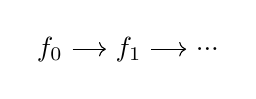
\begin{tikzpicture}
      % Define the nodes
      \node (a) at (0, 0) {$f_0$};
      \node (b) at (1, 0) {$f_1$};
      \node (dots) at (2, 0) {$...$};

      % Draw the arrows
      \draw[->] (a) -- (b);
      \draw[->] (b) -- (dots);
      \end{tikzpicture}
    \end{center}
Counterexample to:
\begin{itemize}
  \item WN
  \item bounded
  \item RP $\implies$ bounded
  \item WCR $\implies$ WN
  \item CR $\implies$ WN
  \item CR and CP $\implies$ WN
  \item CR and CP $\implies$ bounded
\end{itemize}

\subsection*{Counterexample 6}
An infinite sequence with a bound that is a normal form.
\begin{center}

  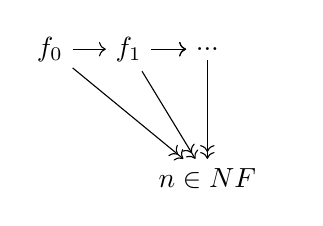
\begin{tikzpicture}
      % Define the nodes inside the region f
      \node (f0) at (0, 0) {$f_0$};
      \node (f1) at (1, 0) {$f_1$};
      \node (dots) at (2, 0) {$...$};

      % Draw the arrows between the nodes inside the region f
      \draw[->] (f0) -- (f1);
      \draw[->] (f1) -- (dots);
      \draw[->] (f1) -- (dots);


      % Define the nodes outside the region f
      \node (a) [below=of dots, yshift=-.25cm] {\parbox{2cm}{\centering $n\in NF$ }};

          % Draw the arrows between the nodes inside and outside the region f sds

          \draw[->>] (f0) -- (a);
          \draw[->>] (f1) -- (a);
          \draw[->>] (dots) -- (a);
      \end{tikzpicture}


    \end{center}
Counterexample to:
\begin{itemize}
  \item WN $\implies$ SN
  \item WN and CR $\implies$ SN
  \item WN, CR, and bounded $\implies$ SN
  \item WN, UN, and bounded $implies$ SN
  \item (Local) WN and UN $\implies$ SR
  \item (Local) WN and NP $\implies$ SR
  \item (Local) WN and RP $\implies$ SR
  \item (Local) WN and CR $\implies$ SR
\end{itemize}

\subsection*{Counterexample 7}
An infinite sequence with a bound that is a normal form where each element
of the sequence has a single step relation to the initial element of the sequence.
\begin{center}
  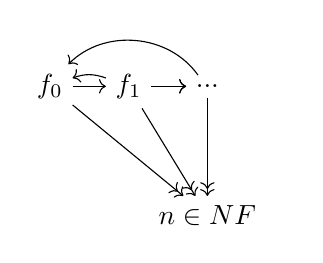
\begin{tikzpicture}
      % Define the nodes inside the region f
      \node (f0) at (0, 0) {$f_0$};
      \node (f1) at (1, 0) {$f_1$};
      \node (dots) at (2, 0) {$...$};

      % Draw the arrows between the nodes inside the region f
      \draw[->] (f0) -- (f1);
      \draw[->] (f1) -- (dots);
      \draw[->] (f1) -- (dots);
      \draw[->] (f1) to [bend right=20] (f0);
      \draw[->] (dots) to [bend right=50] (f0);



      % Define the nodes outside the region f
      \node (a) [below=of dots, yshift=-.25cm] {\parbox{2cm}{\centering $n\in NF$ }};

          % Draw the arrows between the nodes inside and outside the region f sds

          \draw[->>] (f0) -- (a);
          \draw[->>] (f1) -- (a);
          \draw[->>] (dots) -- (a);
      \end{tikzpicture}


    \end{center}
Counterexample to:
\begin{itemize}
  \item RP
\end{itemize}

\subsection*{Counterexample 8}
An "infinite haircomb"
\begin{center}
  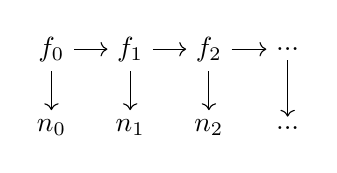
\begin{tikzpicture}
      % Define the nodes inside the region f
      \node (f0) at (0, 0) {$f_0$};
      \node (f1) at (1, 0) {$f_1$};
      \node (f2) at (2, 0) {$f_2$};
      \node (dots) at (3, 0) {$...$};

      \node (n0) at (0, -1) {$n_0$};
      \node (n1) at (1, -1) {$n_1$};
      \node (n2) at (2, -1) {$n_2$};
      \node (dots2) at (3, -1) {$...$};

      \draw[->] (f0) -- (f1);
      \draw[->] (f1) -- (f2);
      \draw[->] (f2) -- (dots);

      \draw[->] (f0) -- (n0);
      \draw[->] (f1) -- (n1);
      \draw[->] (f2) -- (n2);
      \draw[->] (dots) -- (dots2);


      \end{tikzpicture}


    \end{center}
Counterexample to:
\begin{itemize}
  \item WN $\implies$ WCR
  \item WN $\implies$ bounded
  \item WN $\implies$ SN
  \item WN and RP $\implies$ SN
\end{itemize}

\subsection*{Counterexample 9}
\begin{center}

  \begin{tikzcd}[node distance=2cm, auto]
      % Nodes
      \node (a) {a};
      \node (b) [right of=a, xshift=1cm] {b};

      % Arrows
      \draw[->] (a) to [bend left] (b);
      \draw[->] (b) to [bend left] (a);
  \end{tikzcd}

\end{center}
Counterexample to:
\begin{itemize}
  \item (Local) WR and UN $\implies$ WN 
  \item (Local) SR and UN $\implies$ WN 
  \item (Local) SR and NP $\implies$ WN 
  \item (Local) SR and RP $\implies$ WN 
  \item (Local) SR and CR $\implies$ WN 
\end{itemize}

\subsection*{Counterexample 10}
\begin{center}
  \begin{tikzpicture}
      % Nodes
      \node (a) {a};
      \node (b) [left of=a, xshift=-1cm, yshift=-1cm] {b};
      \node (c) [left of=b] {c};
      \node (f0) [right of=a, xshift=1cm, yshift=-1cm] {$f_0$};
      \node (f1) [right of=f0, xshift=1cm] {$f_1$};
      \node (f2) [right of=f1, xshift=1cm] {$f_2$};
      \node (dots) [right of=f2, xshift=1cm] {...};
      
      % Arrows
      \draw[->] (a) -- (b);
      \draw[->] (b) to [bend left] (c);
      \draw[->] (c) to [bend left] (b);
      \draw[->] (a) -- (f0);
      \draw[->] (f0) -- (f1);
      \draw[->] (f1) -- (f2);
      \draw[->] (f2) -- (dots);
  \end{tikzpicture}
\end{center}

Counterexample to:
\begin{itemize}
  \item (Local) WR and NP $\implies$ RP 
\end{itemize}

\subsection*{Counterexample 11}
\begin{center}
  \begin{tikzpicture}
      % Nodes
      \node (a) {a};
      \node (b) [left of=a, xshift=-1cm, yshift=-1cm] {b};
      \node (c) [left of=b] {c};
      \node (d) [right of=a, xshift=1cm, yshift=-1cm] {d};
      \node (e) [right of=d] {e};
      
      % Arrows
      \draw[->] (a) -- (b);
      \draw[->] (b) to [bend left] (c);
      \draw[->] (c) to [bend left] (b);
      \draw[->] (a) -- (d);
      \draw[->] (d) to [bend left] (e);
      \draw[->] (e) to [bend left] (d);

  \end{tikzpicture}
\end{center}

Counterexample to:
\begin{itemize}
  \item (Local) SR and NP $\implies$ RP 
\end{itemize}



\section{Well-foundedness}
\subsection{Well-foundedness}
\sacomment{Talk about the different types of wellfoundedness, starting with the one given in the book, the reason for thinking it is classical and not constructive, and provide an image showing the relation between the notions of wellfoundedness we have. Talk about future work in this area.}

\apcomment{Mention that, for a set $A$, we will use "subset of $A$" and "predicate on $A$" interchangeably,
with subsets being represented in the Agda code using predicates, which are in turn formalized as
dependent types over $A$, i.e. maps $\phi : A \to \bset$ }

Working in constructive logic introduces subtle differences between notions of well-foundedness of relations
which are not present in classical logic.  In our investigation, we have focused on four distinct definitions of well-foundedness, with minor variations of each. To spell these out, we first define some preliminary notions.
% The make clear the difference between these distinct notions of well-foundedness we first present the following defintiions for a given relation $R$.

\begin{dfn} Let $A$ be a set and $R \sse A \times A$ be a relation.
\begin{enumerate}
  \item Let $\phi$ be a predicate on $A$. An element $x \in A$ is $R$-minimal for $\phi$ if $\phi(x)$ is true and no other element for which $\phi$ holds is $R$-related to $x$.
  \item An element $x \in A$ is \textit{$R$-accessible} if every element $R$-related to $x$ is \textit{$R$-accessible}.  (This should be understood as an inductive definition, with base case consisting of $R$-minimal elements for the whole of $A$.)
    \item A predicate $\phi$ on $A$ is \emph{inductive} if it holds on a given element $x \in A$ whenever it holds on all elements $R$-related to $x$:
    \[ (\forall y. Ryx \to \phi(y)) \to \phi(x) \]
    \item A sequence $s = (s_0,s_1,\dots)$ of elements of $A$ is $R$-decreasing
    if every element is related to its predecessor.  That is, $Rs_{n+1}s_n$ for all $n$.
\end{enumerate}
\end{dfn}
With the above definitions established we define the notions of well-foundedness we have been investigating.
\begin{dfn} \hfil
  \begin{enumerate}
    \item \textit{R} is well-founded if every element is \textit{R}-accessible.
    \item \textit{R} is well-founded if every inductive predicate is universally true.
    \item \textit{R} is well-founded if every non-empty predicate has a minimal element with respect to $R$.
    \item \textit{R} is well-founded if every sequence contains a non-decreasing index.
  \end{enumerate}
\end{dfn}
  Further, we explored weaker variants of these notions of well-foundedness.
  \begin{dfn} \hfil
    \begin{enumerate}
      \item \textit{R} is well-founded if every element is $\lnot \lnot$  \textit{R}-accessible.
      \item \textit{R} is well-founded if for every inductive predicate $\phi$, $\lnot \lnot \phi$ is universally true.
      \item \textit{R} is well-founded if it is not not the case that every non-empty predicate has a minimal element with respect to $R$. \textcolor{red}{is there a better way to express this double negation in english?}
      \item \textit{R} is well-founded if there is no infinite $R$-decreasing sequence (this is the definition of well-foundedness found in TeReSe).
    \end{enumerate}
\end{dfn}

\begin{figure}[h]
  \centering
  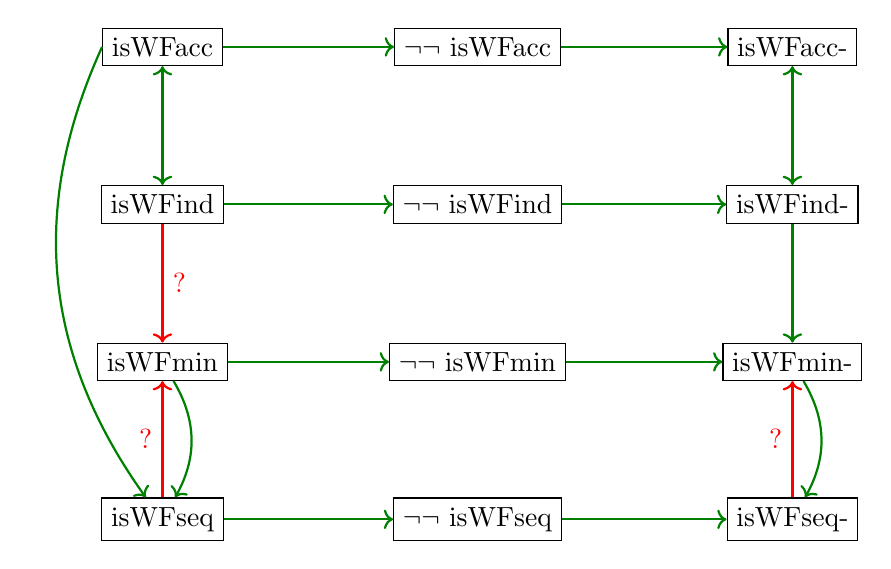
\begin{tikzpicture}[node distance=2cm, auto]
    % Standard definitions
    \node (std1) [draw] {isWFacc};
    \node (std2) [below of=std1, draw] {isWFind};
    \node (std3) [below of=std2, draw] {isWFmin};
    \node (std4) [below of=std3, draw] {isWFseq};

    % Double negation definitions
    \node (dn1) [right of=std1, xshift=2cm, draw] {$\lnot \lnot$ isWFacc};
    \node (dn2) [right of=std2, xshift=2cm, draw] {$\lnot \lnot$ isWFind};
    \node (dn3) [right of=std3, xshift=2cm, draw] {$\lnot \lnot$ isWFmin};
    \node (dn4) [right of=std4, xshift=2cm, draw] {$\lnot \lnot$ isWFseq};

    % Weaker definitions
    \node (weak1) [right of=dn1, xshift=2cm, draw] {isWFacc-};
    \node (weak2) [right of=dn2, xshift=2cm, draw] {isWFind-};
    \node (weak3) [right of=dn3, xshift=2cm, draw] {isWFmin-};
    \node (weak4) [right of=dn4, xshift=2cm, draw] {isWFseq-};

    % Arrows
    \draw[->, thick, darkgreen] (std1) -- (dn1);
    \draw[->, thick, darkgreen] (std1.west) to[out=180, in=90, bend right] (std4);
    \draw[->, thick, darkgreen] (dn1) -- (weak1);
    \draw[<->, thick, darkgreen] (std1) -- (std2);
    \draw[->, thick, darkgreen] (std2) -- (dn2);
    \draw[->, thick, darkgreen] (dn2) -- (weak2);
    \draw[<->, thick, darkgreen] (weak1) -- (weak2);
    \draw[->, thick, red] (std2) -- (std3) node[pos=0.5, right, red] {?};
    \draw[->, thick, darkgreen] (std3) -- (dn3);
    \draw[->, thick, darkgreen] (dn3) -- (weak3);
    \draw[->, thick, darkgreen] (weak2) -- (weak3);
    \draw[->, thick, darkgreen, bend left] (std3) to (std4);
    \draw[->, thick, darkgreen, bend left] (weak3) to (weak4);
    \draw[->, thick, darkgreen] (std4) -- (dn4);
    \draw[->, thick, darkgreen] (dn4) -- (weak4);
    \draw[->, thick, red, bend left] (std4) -- (std3) node[pos=0.5, left, red] {?};
    \draw[->, thick, red, bend left] (weak4) -- (weak3) node[pos=0.5, left, red] {?};
  \end{tikzpicture}
  \caption{A graphic illustrating the implications we have found between the above
  definitions and those we are still seeking to find. Green arrows indicate that one
  definition implies another, red arrows indicate that we believe an implication should
  be possible but we have not yet found it.
  }
\end{figure}


  As future work we want to know whether the missing implications can be found, or what the minimal additional requirements are for making those implications.

\subsection{Additional Remarks}

\texttt{isWFmin} is only provably when restricted to \emph{decidable} predicates, and this
restriction is also necessary: in general, WFmin for all P implies all predicates are decidable.

  \section{Open Questions }
  \begin{enumerate}
    \item Complete the Wellfoundedness implications:
       \[ WNg \land UN \to CRelem :
       \forall (R : \mathscr{R} A) \to WN R \to \forall x \to is R -UN x \to is R -CR x \]
       \item $WN R \to UN R \to \omega-bdd R \to SN R$ (1.2.3.ii-)
        \item Finish formulating the ``compactness property".  Two candidates:
         \item ``Every cocone for a given infinite sequence loops back to some point in the sequence"
         \item ``If an $R^*$-sequence has a cocone then it's constant after some point on.''
         \item is $\omega$-bounded implied by WN and the following confluence property:
         $a \to^* n \in NF$, and $a \to b$ then $b \to^* n $.
    \item (2024.10.10) Is being $R$-WN inductive?
    \item (2024.10.10) Does $R$ being finitely branching imply
     that, for an inductive $\phi$, if $\lnot \phi(x)$ then
     $\exists y. Rxy \land \lnot \phi(y)$?

    \item If WCR holds, is WN$\downarrow\subseteq$WN ?
    \item Same question for next bullet in 2.2
    \item Same for bullet 3 in 2.2 (but pointwise!)
    \item \item Look at restricting WFmin to $\lnot\lnot$-closed predicates
    \item Status of important hypotheses:
      \begin{itemize}
        \item Deciding whether a given element $x$ reduces to a given element $y$
        (Is $R$ itself decidable?)
        \item Deciding whether a given element $x$ reduces to some element $y$
        (Is being an $R$-normal form decidable?)

        {\textcolor{red}{This is needed to show that SN $\Rightarrow$ WN.}}

        \item If a given element $x$ is \emph{not} a normal form,
        exhibiting some element $y$ that it reduces to.
        (This is related to DeMorgan/Markov/etc. properties that came up in WF file.)

        \item Does UN-lemma \emph{require} the decidability assumption?
      \end{itemize}
    \item META questions: Which of the ARS theorems can be made ``local/pointwise'',
    for example,
    \begin{itemize}
      \item NL+: $WCR(R) \land SN(x) \to CR(x)$?  (Yes?)
      \item NL++: $WCR(x) \land SN(x) \to CR(x)$? (No.)
    \end{itemize}
    \item Can "sequential" properties like RP, RP-, isWFseq, isWFseq-, $\omega$-bounded, etc.,
      be related to the cofinality property.
      \item What happens if properties involving sequences are reformulated for
    $R^r$? (Cannot decide whether the given sequence is finite or infinite.)
    \item Knaster-Tarski Lemma: Most general form? Alternative formulations?
    \item Knaster--Tarski in a well-founded setting: what additional
    hypotheses are necessary?
    \item Show SN and WNFP $\to$ CR : SN R $to$ WNFP R $to$ CR R (or, what combination of properties with WNFP gets us to CR)
    \item Major: Find a classical or constructive solution to theorem 1-2-3 ii. Note, we have a counterexample showing that we
    cannot solve this whilst using recurrence property and boundedness rather than ind(uctive) and inc(reasing). The counterexample is the self loop on an element.
    \item is $\omega$-bounded implied by WN and the following confluence property:
    $a \to^* n \in NF$, and $a \to b$ then $b \to^* n $. (This is a weaker form of WNFP)
    \item WN and WCR $\to$ bounded. We reached a dead end trying to show this before. Check github history in the ARS file for iii-lemma
    if you'd like to see the previous direction.
  \end{enumerate}

  \subsection*{Questions about Well-foundedness}
  \begin{enumerate}
    \item For a given element $x$, is the property of
    being accessible $\lnot\lnot$-closed? I.E.,
    Does $x$ being $\lnot\lnot$-accessible imply that $x$ is accessible?
    (Conjecture: No.)

    \item As a special case, does being weakly (accessible) well-founded imply being $\lnot\lnot$-wellfounded?
    (Conjecture: No.)

    Also: Same question about inductive notion of well-foundedness.

    \item ($\star$) Given a well-founded relation, does every non-empty subset
    have a minimal element?

    \emph{Problem.} Need to decide whether, for a given $x \in U$,
     the set $\{y | Ryx\}$ is empty.

     \item IF every non-empty subset has a minimal element, does this imply
     either of the weak forms of well-foundedness: $\mathtt{isWFacc-}$ or
     $\mathtt{isWFind-}$ ?

     \item Does $\mathtt{isWFmin-}$ imply $\mathtt{isWFacc-}$ or $\mathtt{isWFind-}$?

     \emph{Problem.} Need to go from $\lnot (\forall y. R y d \to \phi y)$
     and $\forall y. R y d \to \lnot \lnot \phi y$ to $\bot$.

     In terms of accessibility, it should suffices to assume accessibility is
     $\lnot\lnot$-closed, since being related to y is not relevant for that. (?)

     \item Does sequential well-foundedness (no decreasing sequence) imply
     any of the other notions, e.g., \texttt{WFmin-} ?

     \emph{Note.}  This seems to require the most classical assumptions:
     $\lnot\lnot$-closure of $\phi$, relativized De Morgan law,
     Markov's principle, etc.
     \textsc{Remark.}
     $\lnot\lnot$-closure of accessibility should solve problems 1 and 4.
  \end{enumerate}
  \newpage

\section{Todo}

\subsection{Main themes}
\begin{enumerate}
  \item Clean up the implications around recurrence properties:
  \begin{itemize}
    \item RP iff cofinality and Boundedness?
    \item What is the ``recurrent'' generalization of WN?
    \item What is the ``recurrent'' generalization of SN?
    \item The role of WCR in the proof of our generalization of Thm. 1.2.3(iii)
  \end{itemize}
  \item Complete the ``design'' of the chart(s) with implications?
  \begin{itemize}
    \item   Look at Exercise 1.3.22 (Show UN $\to$ UN$^\to$ but not conversely. Show a counterexample to WCR and UN$^\to$ $\to$ UN. Find a counter example to WCR and WN $\to$ Ind)
  \end{itemize}
  \item Complete the proof of Theorem 1.2.3
  \item Address outstanding questions about wellfoundness implications.
  \begin{itemize}
    \item WFseq implies WFmin? (Assuming decMin)
    \item WFacc implies $WFmin_0$? (Assuming decMin)
    \item DecMin suffices for $SN\to WN$, but what is the optimal \emph{necessary} condition?
    \item Relationship between these, and De Morgan's laws.
  \end{itemize}
  \item Complete the classical properties section
  \item Complete the guide to the code section
  \item Miscellaneous
  \begin{itemize}
    \item   Make the first argument to "being a normal form" implicit?
    \item   Define: Inc in report
    \item   Define: Ind in report
    \item   Define: $\mathrm{CR}^{\le 1}$ in report
    \item   More laws about closure operations: Monotonicity, idempotency
    \item   Tidy up and standardize the notation used in ars.agda and other agda files
  \end{itemize}
\end{enumerate}

\subsection{12.23}
\begin{enumerate}
  \item Prove isWFseq implies isWFmin1
\end{enumerate}


\subsection{General todo list}
\begin{enumerate}
  \item  Another interesting one? $WN^*$: hereditarily $WN$ ($WN$ for the reduction graph starting from a given element $x$). Could even consider $SN^*$, $CR^*$ etc. \sacomment{Is this what we have already shown
  in the reduction closure properties? If so we can delete this. If not it should be moved to open questions}
\end{enumerate}

\apcomment{For a property $P(x)$, let $\down{P}(x) := \forall y. x \thra y \implies P(y)$}

Note that $\down{P} \subseteq P$.

If the converse inclusion holds, we will say that $P$ is \emph{closed under reduction}.

\newpage

\section{Misc. Notes}


\subsection*{November 21}
\apcomment{These may be addressed by the implications table}
Four local ``normal form properties'':
\begin{enumerate}
  \item $WNFP(a) : \forall n \in NF. (a \tto n) \to \forall b. (a \tto b) \to (b \tto n)$
    "$a$ all reducts of $a$ reduce to $a$'s normal form, if it exists``
  \item $NFP(a) : \forall n \in NF. (a \tto n) \to \forall b. (a \thlra b) \to (b \tto n)$
    "$a$ all converta of $a$ reduce to $a$'s normal form, if it exists``
  \item $WUN(a) : \forall n m \in NF. (a \tto n) \to (a \tto m) \to n \equiv m$
    "$a$ is reducible to at most one normal form"
  \item $UN(a) : \forall n m \in NF. (a \thlra n) \to (a \thlra m) \to n \equiv m$
    "$a$ is convertible to at most one normal form''
\end{enumerate}


\subsection*{Additional remarks about Theorem 1.2.3.}
\begin{itemize}

  \item The goal \texttt{iii-lemma :  $WN(R) \to WCR(R) \to \omega{-}\text{bounded}(R)$}
  seems either very difficult or impossible.

  \apcomment{This implication should be either proved or refuted.}

  Yet, constructing the bound of a given $R$-increasing sequence is key to the proof of
  (our interpretation of) Theorem 1.2.3(iii), namely that
  \[ WN(R) \land WCR(R) \land RP(R) \to SN(R) \tag{iii} \]
  \item Here is a classical proof of this implication.

  Let $R \subseteq A \times A$, and suppose $R$ satisfies WN, WCR, and RP.

  Suppose $R$ is not SN.  Let $a \in A$ be not SN.  By WN, let $n \in \NF$ be
  such that $a \to^* n$.  By induction on the length of this reduction, the finite sequence
  of terms comprising it must contain a final term with the property that
  it is not SN.  (For $n$ is SN, being a normal form, while $a$ is not.)

  $(\star)$ Let this last non-SN term be denoted $b_0$.

  If each single-step $R$-reduct of $b_0$ is SN (so that $b_0 \to x$ implies $x\in \SN$),
  then $b_0$ would itself be SN --- which it is not, by how it was chosen.

  Thus there exists a $c_0$ with $b_0 \to c_0$, and $c_0 \notin \SN$.

  So we have $c_0 \from b_0 \to m_0$ for some $m_0 \in \SN$. ($m_0$ is the next term after $b_0$ in the reduction $a \to^* n$.)

  By WCR, there exists another element $d_0 \in A$ with $c_0 \to^* d_0 \from^* m_0$.

  Since $m_0 \in \SN$ and this set of terms is closed under reduction, $d_0 \in \SN$ as well.

  Thus $b_0 \to c_0 \to^* d_0$, with $d_0 \in \SN$, and $c_0 \notin \SN$.

  Again, the reduction $c_0 \to^* d_0$ contains a last term that is not in SN.

  Let this term be denoted by $b_1$, and let the next term in the reduction sequence
  to $d_0$ be denoted $m_1$.

  Now repeat the above process starting at $(\star)$, incrementing all subscripts by 1.

  This generates an infinite reduction sequence

  \[b_0 \to c_0 \to^* b_1 \to c_1 \to^* b_2 \to \cdots \]

  Note that infinitely many terms in this sequence are one reduction step
  away from a term in $\SN$.

  Moreover, notice that the normal forms of $m_0$, $d_0$, and $m_1$ are the same
  and equal to $n$, whence the same is true for $m_1$, $d_1$, and $m_2$, etc.

  It follows that, for infinitely many terms in the sequence
  (namely, all the terms $b_i$), we have $b_i \to^* n$.

  Thus, all terms in the sequence reduce to $n$ and so $n$ is an $\omega$-bound
  of the sequence.

  By RP, some term $r$ in the sequence is recurrent.

  Since $r \to^* n$ and $r$ is recurrent, also $n \to^* r$.

  But $n$ is a normal form.  So this sequence is empty and $r=n$.

  But $r$ is a term in an infinite reduction sequence, and reduces to its successor.

  This yields a contradiction.

\end{itemize}



\end{document}
